
\documentclass[12pt,twocolumn,twoside]{article}
\usepackage{lingmacros}
\usepackage{tree-dvips}
\usepackage{graphicx}
\usepackage{caption}
\usepackage{subcaption}

\graphicspath{ {./img/} }

\begin{document}
	
	\title{Visual Analytics \\
		\large Engineering in Computer Science - Sapienza\\ Class 2019-2020}
	
	
	\author{Matteo Rizza, Nicola Di Santo}

	\twocolumn[
		\begin{@twocolumnfalse}
			\maketitle
			\begin{abstract}
				The main goal of this application is to allow users to visualize the genes interaction of available diseases. A set of filters and live analytics are provided  that theoretically should allow user to better understand genes interaction and consequently formulate or validate hypothesis in the emerging field of network medicine. \\
				We are strongly inspired by the NEMESIS \cite{ivapp19} system but we adopted a slightly different approach by using a classic and widely used node-link diagram for displaying the interactome as well as a different kind of insights to the user.\\ For the realization of the whole visual part the \emph{d3.js}\cite{d3} library is used.
			\end{abstract}
		\end{@twocolumnfalse}
		]
%Image of the system here
 

\section*{Introduction}
The emerging tools of network medicine offer a platform to explore systematically not only the molecular complexity of a particular disease, leading to the identification of disease modules and pathways, but also the molecular relationships among apparently distinct phenotypes. Advances in this direction are essential for identifying new disease genes, for uncovering the biological significance of disease-associated mutations identified by genome-wide association studies and full-genome sequencing, and for identifying drug targets and biomarkers for complex diseases. This project tries to provide an interactive visual system to allow operator to navigate and process this huge amount of graph structured data to allow them to formulate or validate new hypothesis.\\ %talk about definitions 

\section*{Dataset} %insert picture of data
The datasets used in this project is from the OMIM (Online Mendelian Inheritance in Man) project. It is a comprehensive, authoritative and timely knowledge-base of human genes and genetic disorders compiled to support human genetics research and education and the practice of clinical genetics. \\
From OMIM data we have used the Interactome Dataset, the Seeds Dataset and the Drug Target Dataset. The Interactome Dataset is a relational dataset made of 141000. Each row is composed by five record, the first two represent a link between two genes expressed as id of source and target genes, the second two are the genes symbols (readable names) while the last one tells how this link was discovered. The Seeds dataset is a key-value dataset with key the name of a disease and with value a list of genes involved in the relative disease. The last one is instead a mapping between drugs and genes it acts on. All those data have been exported from Excel format to TSV format and subsequently loaded into our application.\\ Since the interactome is very huge, to speedup the computations it is filtered and only links with source or target involved in at least one disease or drug are selected. This operation allows us to reduce its size of 70\% speeding up all the subsequent filtering necessary for visualization. The cut interactome dataset has $39000$ tuples, so even with this huge shrinking of interactome size and without considering the other datasets  we still respect requirements of $AS-index > 10000$ .

\section*{The System}
The system is composed of three main visualizations plus some filter components. When it is loaded for the first time only Diseases Scatterplot View and sidebar with filters are visible, all the other views depends on user selection.\\ 
The user is allowed to select at most five diseases. To select a disease to analyze, he can use interchangeably either the scrollable sidebar on the right side of the screen or the scatterplot on the left upper corner of the screen. According to this selection the interactome node-link diagram is displayed. Once the interactome network graph is visible the user is allowed to select a drug and understand if there is some gene of the interactome affected by that drug. Top 5 centrality genes are also computed for the interactome of selected diseases and they are displayed to the user in left lower corner.
\subsection*{Diseases Scatterplot View}
The Disease Scatterplot view is a scatterplot showing all the available disease to analyze\ref{scatter}. Each disease is represented as a point. Each point has a $0.5$ opacity to make overlapping points visible. The view is zoomable so that very near points can be distinguished and further analyzed. The axes, representing distances between points in the x and y reference frame are scaled according to the zoom to make user understand the degree of similarity between points.\\ 
To draw diseases as 2-D points we have, first of all, defined a distance measure between them. The distance is defined using Jaccard Similarity on the genes involved in the disease. Namely if we have two diseases $D_i$ and $D_j$ with $D_i$ acting on genes $G_i=\{g_{i1},g_{i2},...,g_{in}\}$ and $D_j$ acting on genes $G_j=\{g_{j1},g_{j2},...,g_{jm}\}$ where $G_j and G_i$ are sets, we can compute the similarity between two disease as the jaccard similarity on their set of genes: $J_s = \frac{|G_i \cap G_j|}{|G_i \cup G_j|}$, the distance is simply $d =1-J_s$.  Then the symmetric distance matrix between diseases is computed and multidimensional scaling (MDS) is applied on it to obtain 2-D points for each disease. We recall that an MDS algorithm places each object into N-dimensional space (N is an input parameter, $N=2$ in our case) such that the between-object distances are preserved as well as possible.\\ MDS is computed at the start-up of the system. We have used algorithm from \cite{mds_js}.

	\begin{figure}
		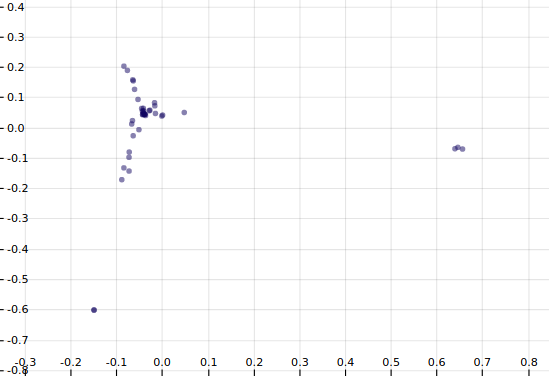
\includegraphics[width=.95\linewidth]{disease-scatterplot-mds.png}
		\caption{Disease scatterplot View}
		\label{scatter}
	\end{figure}
This view is coordinated to the Diseases Interactome View and the sidebar disease selector in the sense that we can choose a disease to display in the interactome node-link diagram by either clicking on the side bar selector or by clicking on a point in the scatterplot. Whenever we click on the sidebar selector entry, a point in the scatterplot corresponding to the selected disease is colored with the same color of the nodes of that disease in the Interactome View. Whenever we click on a scatterplot disease, the corresponding disease's nodes are drawn in the Interactome graph and the disease entry in the sidebar selector is focused in green.\\ The view can also be considered indirectly connected to the Top 5 Centrality View, since it triggers an Interactome change that on its own side triggers changes on the Top 5 Centrality View. \\To provide a better understanding of the scatterplot, by hovering a point with the mouse, a tooltip with the name of the corresponding disease is displayed. 
\subsection*{Diseases Interactome View}
\subsection*{Top 5 Centrality View}
\subsection*{Coordination Between Views}




\clearpage
\bibliographystyle{unsrt}
\bibliography{citazioni} 

\end{document}